\documentclass{beamer}
\usepackage[utf8]{inputenc}
\usepackage{graphicx}
\usepackage{color}

\usetheme{Warsaw}

\title{TeXloud, le \LaTeX \ dans le cloud}
\author[Bruyère, Ducatel, Rakotondratsima, Biha, Bouchakor]{Adrien Bruyère,\\David Ducatel, Meva Rakotondratsima,\\Sidina Biha, Zakaria Bouchakor}
\institute{Université du Havre}
\date{24 Février 2011}

%numerotation des slides
\defbeamertemplate*{footline}{shadow theme}
{%
  \leavevmode%
  \hbox{\begin{beamercolorbox}[wd=.5\paperwidth,ht=2.5ex,dp=1.125ex,leftskip=.3cm plus1fil,rightskip=.3cm]{author in head/foot}%
    \usebeamerfont{author in head/foot}\insertframenumber\,/\,\inserttotalframenumber\hfill\insertshortauthor
  \end{beamercolorbox}%
  \begin{beamercolorbox}[wd=.5\paperwidth,ht=2.5ex,dp=1.125ex,leftskip=.3cm,rightskip=.3cm plus1fil]{title in head/foot}%
    \usebeamerfont{title in head/foot}\insertshorttitle%
  \end{beamercolorbox}}%
  \vskip0pt%
}

% supprime les outils de navigation en bas a droite
\setbeamertemplate{navigation symbols}{}


%changement des couleur
\definecolor{disablePuce}{rgb}{0.20,0.43,0.09}  % vert fonce
\definecolor{background}{rgb}{0.20,0.43,0.09}

\setbeamercolor{subsection in head/foot}{fg=white, bg=black}
\setbeamercolor{section in head/foot}{fg=white, bg=background!75!black}

\setbeamercolor{structure}{fg=black, bg=disablePuce!40}
%%%%%%%%%%%%%%%%%%%%%%%%%%%%%%fin du préambule%%%%%%%%%%%%%%%%%%%%%%%%%%%%%%%%%%%%%%%%%%%%%%%%%%%%%%%%%%%%%%

\begin{document}

\begin{frame} %%%page de presentation
  \titlepage
\end{frame}


\AtBeginSection[] %%ici pour le plan
{
  \begin{frame}<beamer>
     \begin{columns}[t]
  \begin{column}{5cm}
  \tableofcontents[sections={1},currentsection, hideothersubsections]
  \end{column}
  \begin{column}{5cm}
  \tableofcontents[sections={2-3},currentsection,hideothersubsections]
  \end{column}
  \end{columns}
  \end{frame}
}

\section{Introduction}
\subsection{\LaTeX}
\begin{frame}{Introduction -- \LaTeX}
	\begin{itemize}
	\item Langage de description de documents.
	\item Publications scientifiques.
	\item Excellent rendu des équations et formules.
	\item Convertible en PDF, PostScript, DVI, HTML , etc.
	\end{itemize}
\end{frame}


\subsection{Projet}
\begin{frame}{Introduction -- Projet}
	\begin{itemize}
	 \item Création de documents \LaTeX.
     \item Plateformes dépourvues de distribution \LaTeX.
     \item Espace de stockage privé.
     \item Forte scalabilité
	\end{itemize}
\end{frame}

\subsection{Environnement}
\begin{frame}{Introduction -- Environnement}
	\begin{block}{Environnement}
		\begin{itemize}
		\item Python
		\item PHP5
		\item JQuery
		\item Mysql
		\item Android
		\item Etc.
		\end{itemize}
	\end{block}
\end{frame}

\subsection{Architecture générale}
\begin{frame}{Introduction -- Architecture générale}
	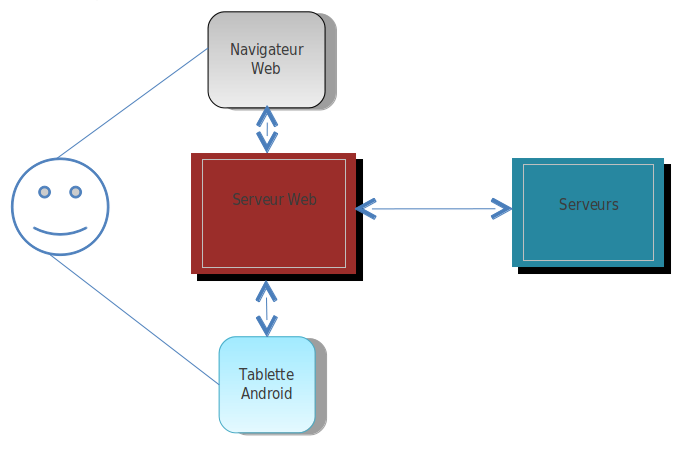
\includegraphics[width=\textwidth]{./images/diaBiha.png}
\end{frame}

\section{Fonctionnement autour d'une compilation}
\subsection{Serveur HTTP}
\begin{frame}{Fonctionnement autour d'une compilation}
 	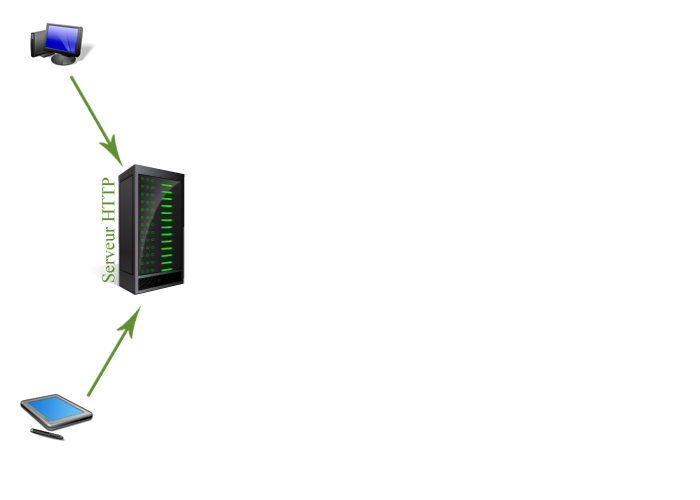
\includegraphics[width=0.95\textwidth]{./images/step1}
\end{frame}
\begin{frame}{Fonctionnement autour d'une compilation}
 	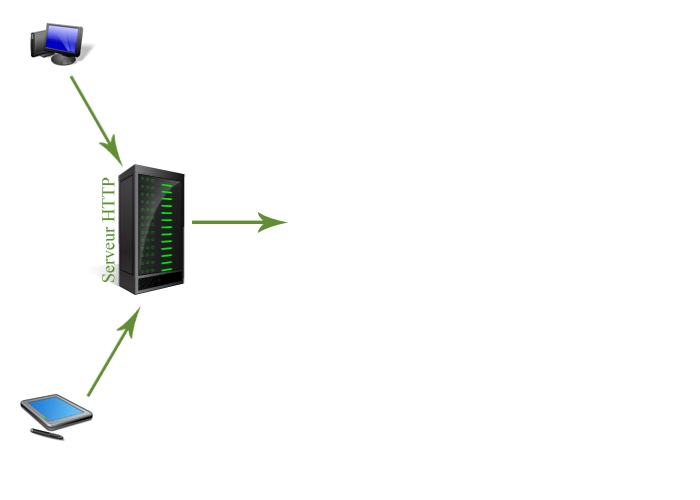
\includegraphics[width=0.95\textwidth]{./images/step2}
\end{frame}

\subsection{Serveur frontal}
\begin{frame}{Fonctionnement autour d'une compilation}
 	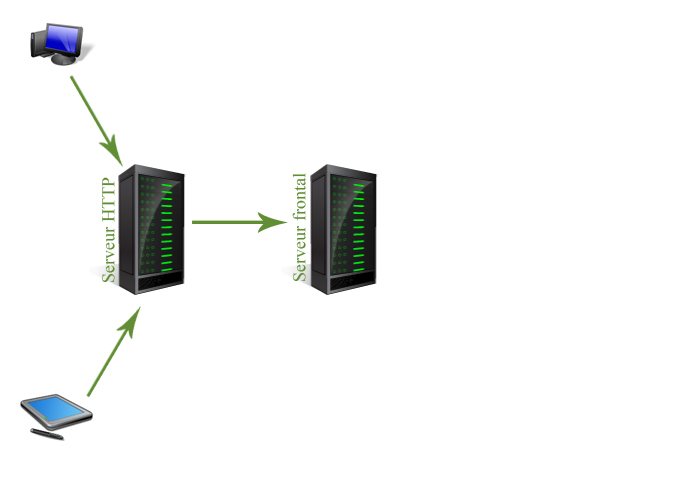
\includegraphics[width=0.95\textwidth]{./images/step3}
\end{frame}
\begin{frame}{Fonctionnement autour d'une compilation}
 	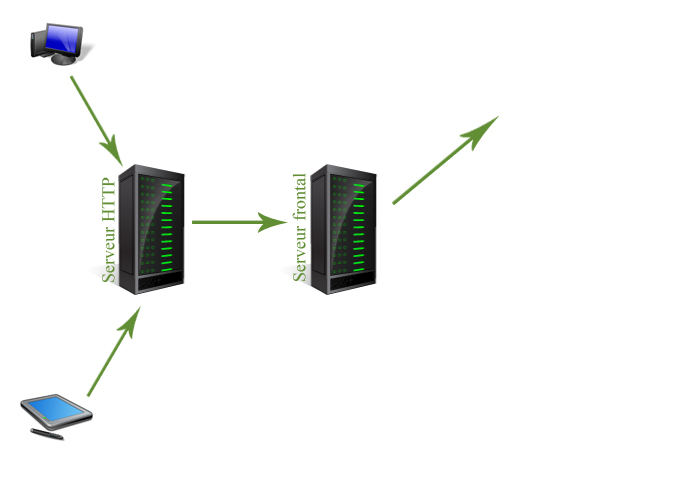
\includegraphics[width=0.95\textwidth]{./images/step4}
\end{frame}

\subsection{Serveurs de données}
\begin{frame}{Fonctionnement autour d'une compilation}
 	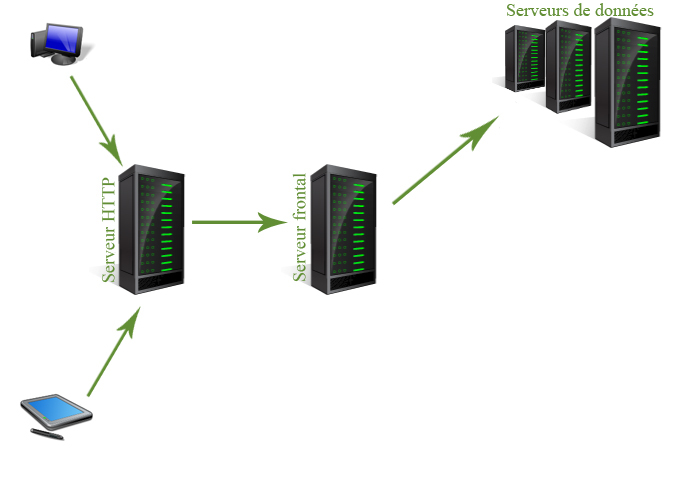
\includegraphics[width=0.95\textwidth]{./images/step5}
\end{frame}
\begin{frame}{Fonctionnement autour d'une compilation}
 	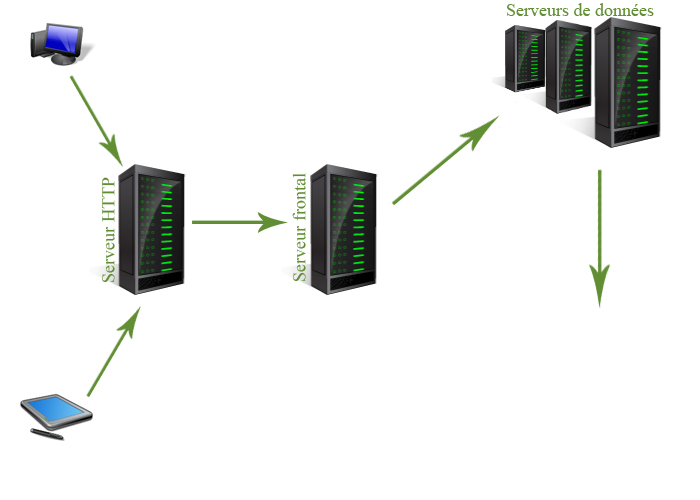
\includegraphics[width=0.95\textwidth]{./images/step6}
\end{frame}

\subsection{Serveurs de compilation}
\begin{frame}{Fonctionnement autour d'une compilation}
 	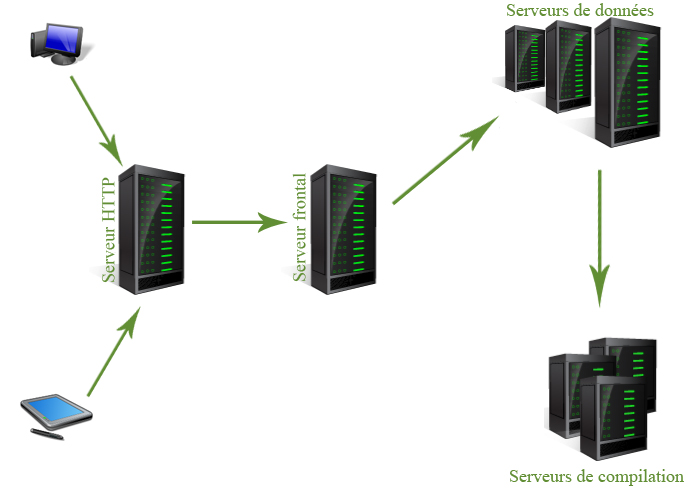
\includegraphics[width=0.95\textwidth]{./images/step7}
\end{frame}
\begin{frame}{Fonctionnement autour d'une compilation}
 	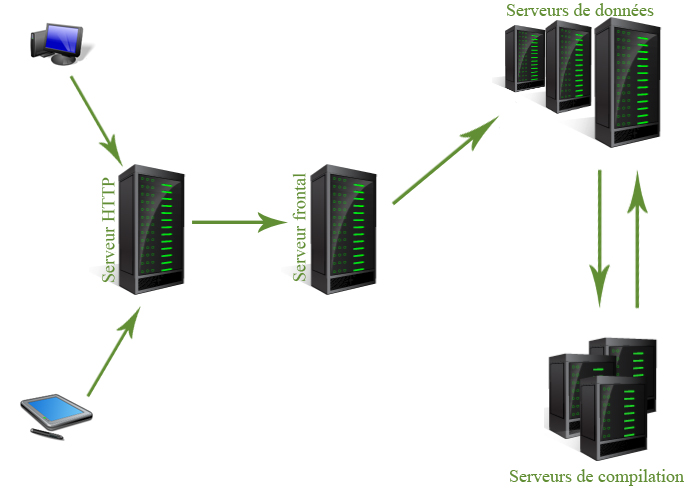
\includegraphics[width=0.95\textwidth]{./images/step8}
\end{frame}

\subsection{Retour au client}
\begin{frame}{Fonctionnement autour d'une compilation}
 	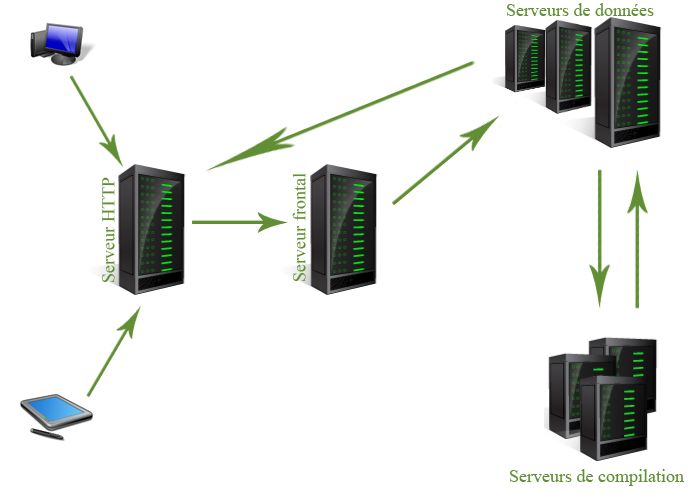
\includegraphics[width=0.95\textwidth]{./images/step9}
\end{frame}
\begin{frame}{Fonctionnement autour d'une compilation}
 	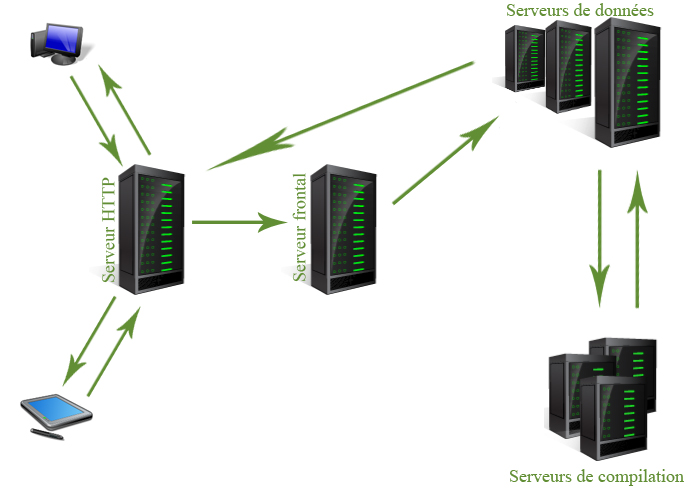
\includegraphics[width=0.95\textwidth]{./images/step10}
\end{frame}

\section{Conclusion}
\begin{frame}
 \begin{figure}
  	
\includegraphics[scale=0.7]{./images/logoTexloud}
	\centering
 \end{figure}
\end{frame}

\end{document}
